\begin{frame}{Analyse différentielle et boomerang}
    \large{\centerline{\textbf{Attaque sur SbPN}}}

\end{frame}

%------------------------------------------------
%------------------------------------------------

\begin{frame}{Le retour de Jafar \FiveStar \FiveStar \hfill \textcolor{red}{8 résolutions :(}}
    \begin{columns}[c]
        \column{.45\textwidth}
        \begin{center}                  
            
\includegraphics[width=0.9\textwidth]{img/meme/jafar-intro.png}
        \end{center}

        \column{.65\textwidth} % 
           \begin{outline}
                \1 Objectifs : 
                    \2 Forger un couple clair / chiffré sans connaître la clef

                    \pause 
                \1 Données
                    \2 Exactement 3 oracles de chiffrement / déchiffrement
                    \2 Le code source
           \end{outline}
    \end{columns}
\end{frame}


%------------------------------------------------
%------------------------------------------------

\begin{frame}{Le cipher Jafar}
  \begin{columns}[c]
        \column{.50\textwidth} %
             \begin{center}                  
                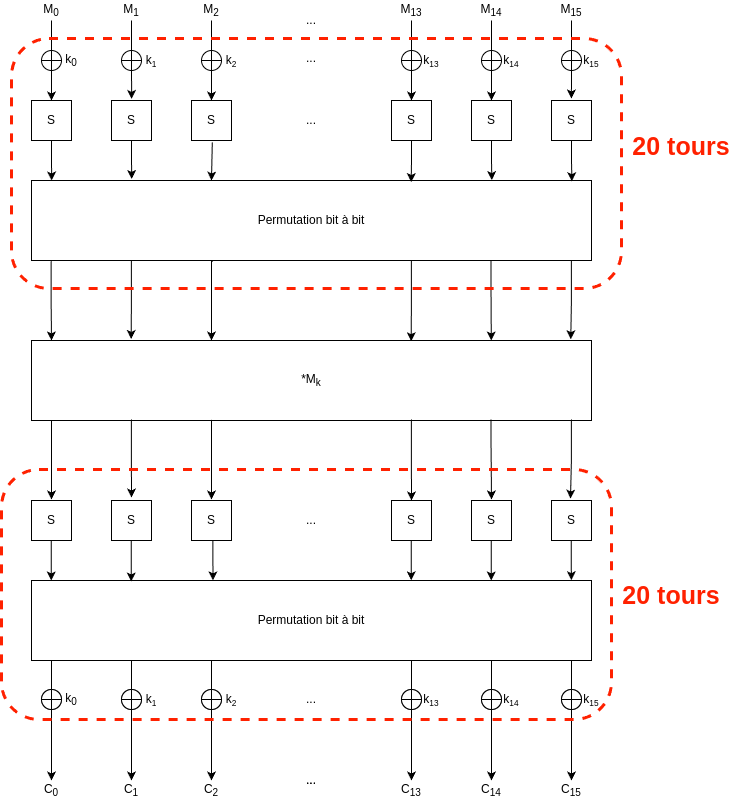
\includegraphics[width=0.9\textwidth]{img/crypto/jafar/jafar-scheme.png}
            \end{center}
        \column{.50\textwidth}
           \begin{outline}
                \1 40 tours au total
                \pause
                \1 Pas de tour de clef
                \pause
                \1 Tout est linéaire à part la SBox
                \pause
                \begin{center}                  
                 
\includegraphics[width=0.9\textwidth]{img/meme/jafar-meme.png}
                \end{center}
                \hfill \tiny{@bluesheet}
           \end{outline}
    \end{columns}
\end{frame}

%------------------------------------------------
%------------------------------------------------

\begin{frame}[fragile] % <---
\frametitle{Fausse piste : la permutation}
  \begin{columns}[c]

    \column{.45\textwidth}
        \begin{lstlisting}[language=Python]
P_Perm = Permutation(P)
P_perm.show("braid")
P_perm.fixed_points()
P_perm.cycle_tuples()
        \end{lstlisting}

        \begin{itemize}
            \item Deux points fixes (2 et 94)
            \item Trois cycles non triviaux de taille 82, 31, 13
        \end{itemize}
    \column{.40\textwidth} %
        \begin{center}                  
            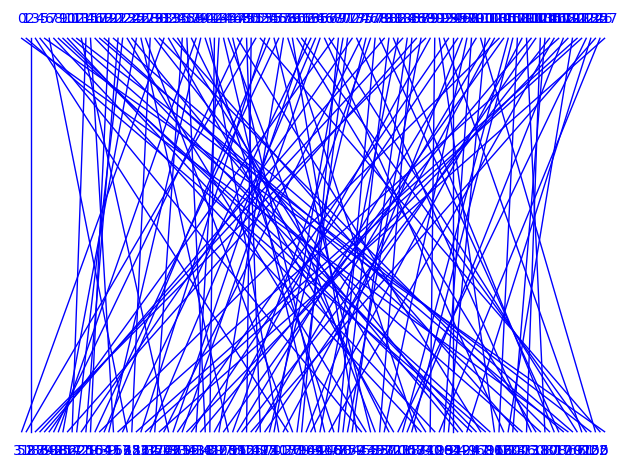
\includegraphics[width=0.9\textwidth]{img/crypto/jafar/permutation.png}
        \end{center}
    \end{columns}

\end{frame}


\begin{frame}[fragile] % <---
\frametitle{Analyse de la SBox}
  \begin{columns}[c]
    \column{.70\textwidth}
        \begin{lstlisting}[language=Python]
from sage.crypto.sbox import SBox
sb = SBox(S)
sb.difference_distribution_table()
\end{lstlisting}
        \begin{outline}
            \1 DDT[a,b] := Probabilité que $S[x\oplus a] = S[x]\oplus b$
            
            \only<2->{
                \2[$\longrightarrow$] 4 différentielles par Sbox: $(0\mapsto 0)$ ,$(24\mapsto 129)$, $(74\mapsto 7)$, $(82 \mapsto 134)$
                }
            \only<3->{
            \1 16 octets $\Rightarrow$ $2^{32}$ différentielles à tester
            }
        \end{outline}
    \column{.30\textwidth} %
        \begin{center}                  
            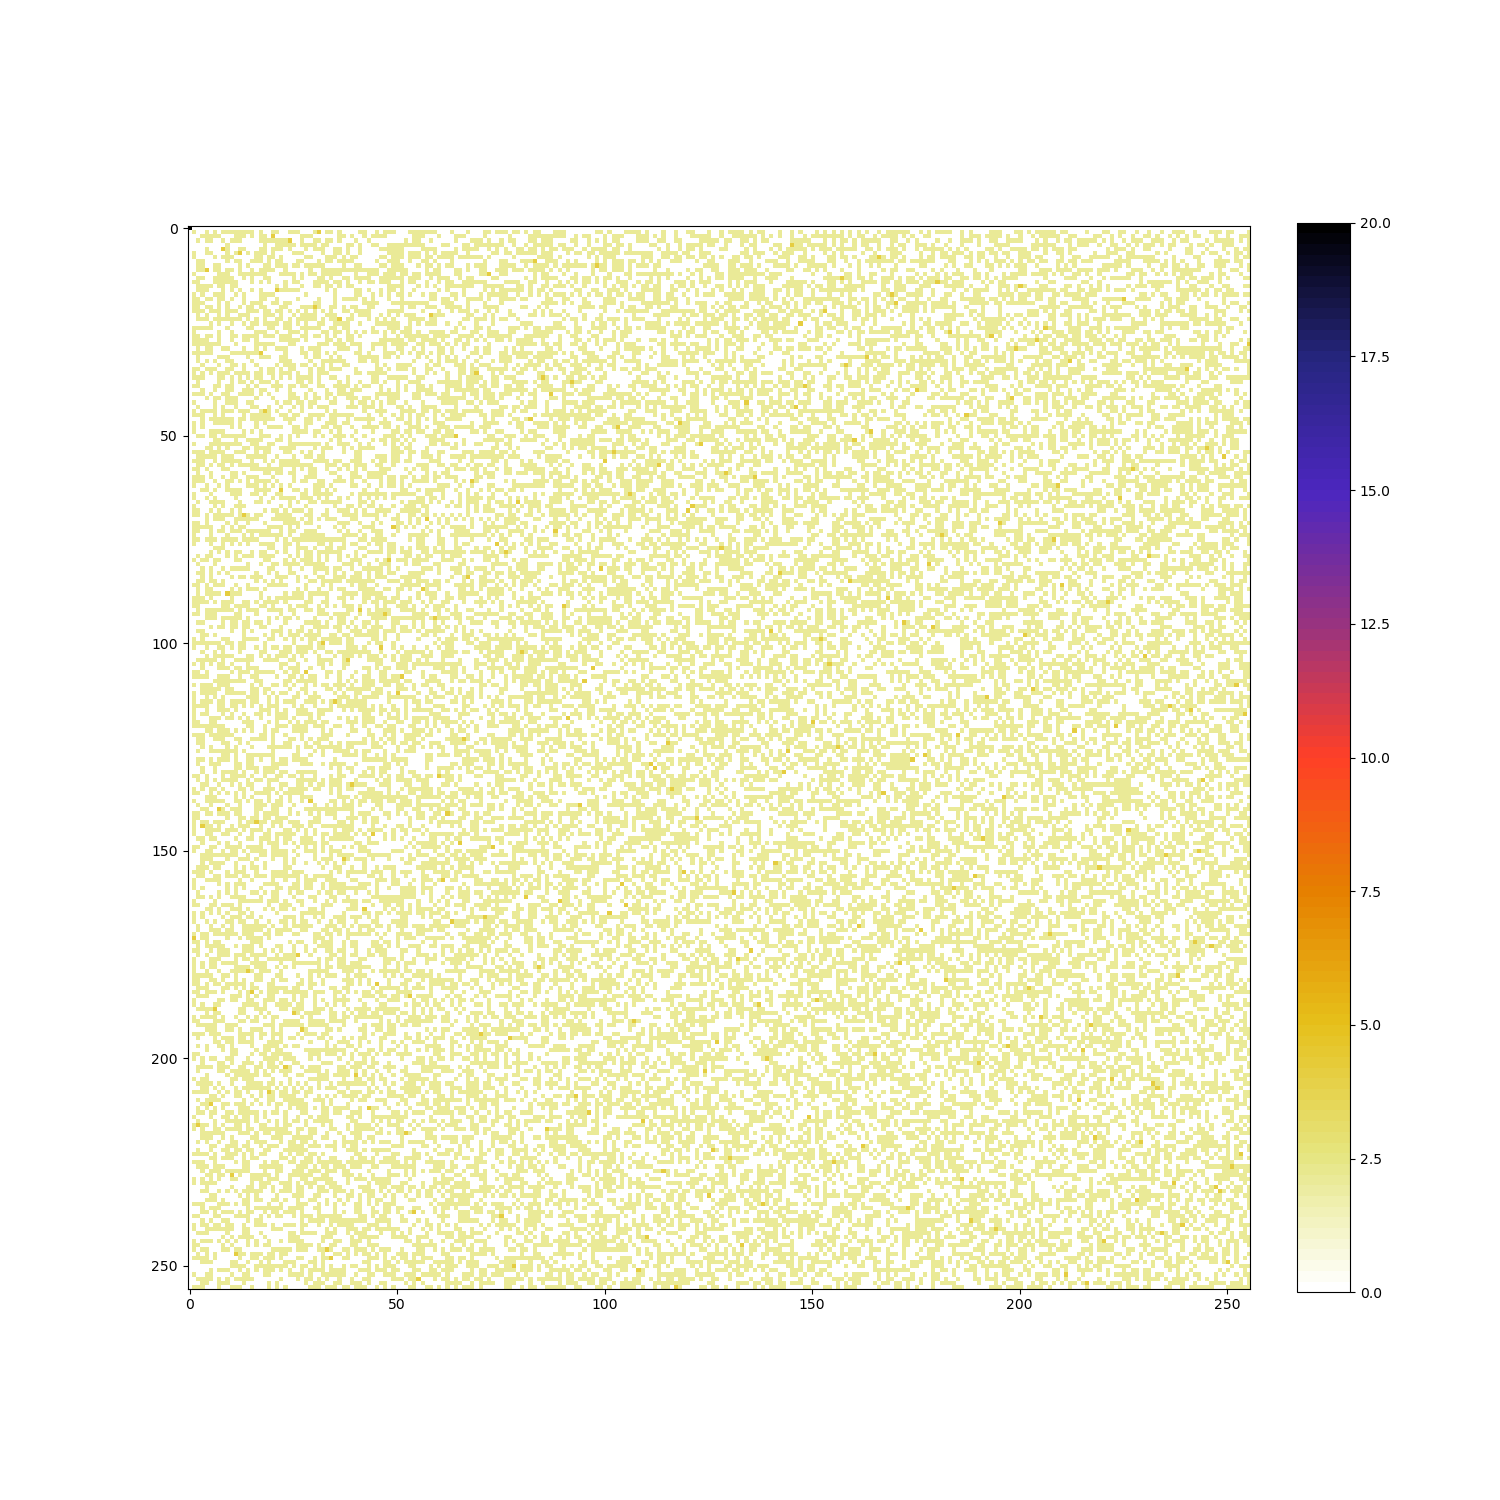
\includegraphics[trim=30pt 140pt 30pt 140pt, clip, width=0.9\textwidth]{img/crypto/jafar/AES-ddt.png}
        \end{center}
        \pause 
        \begin{center}                  
            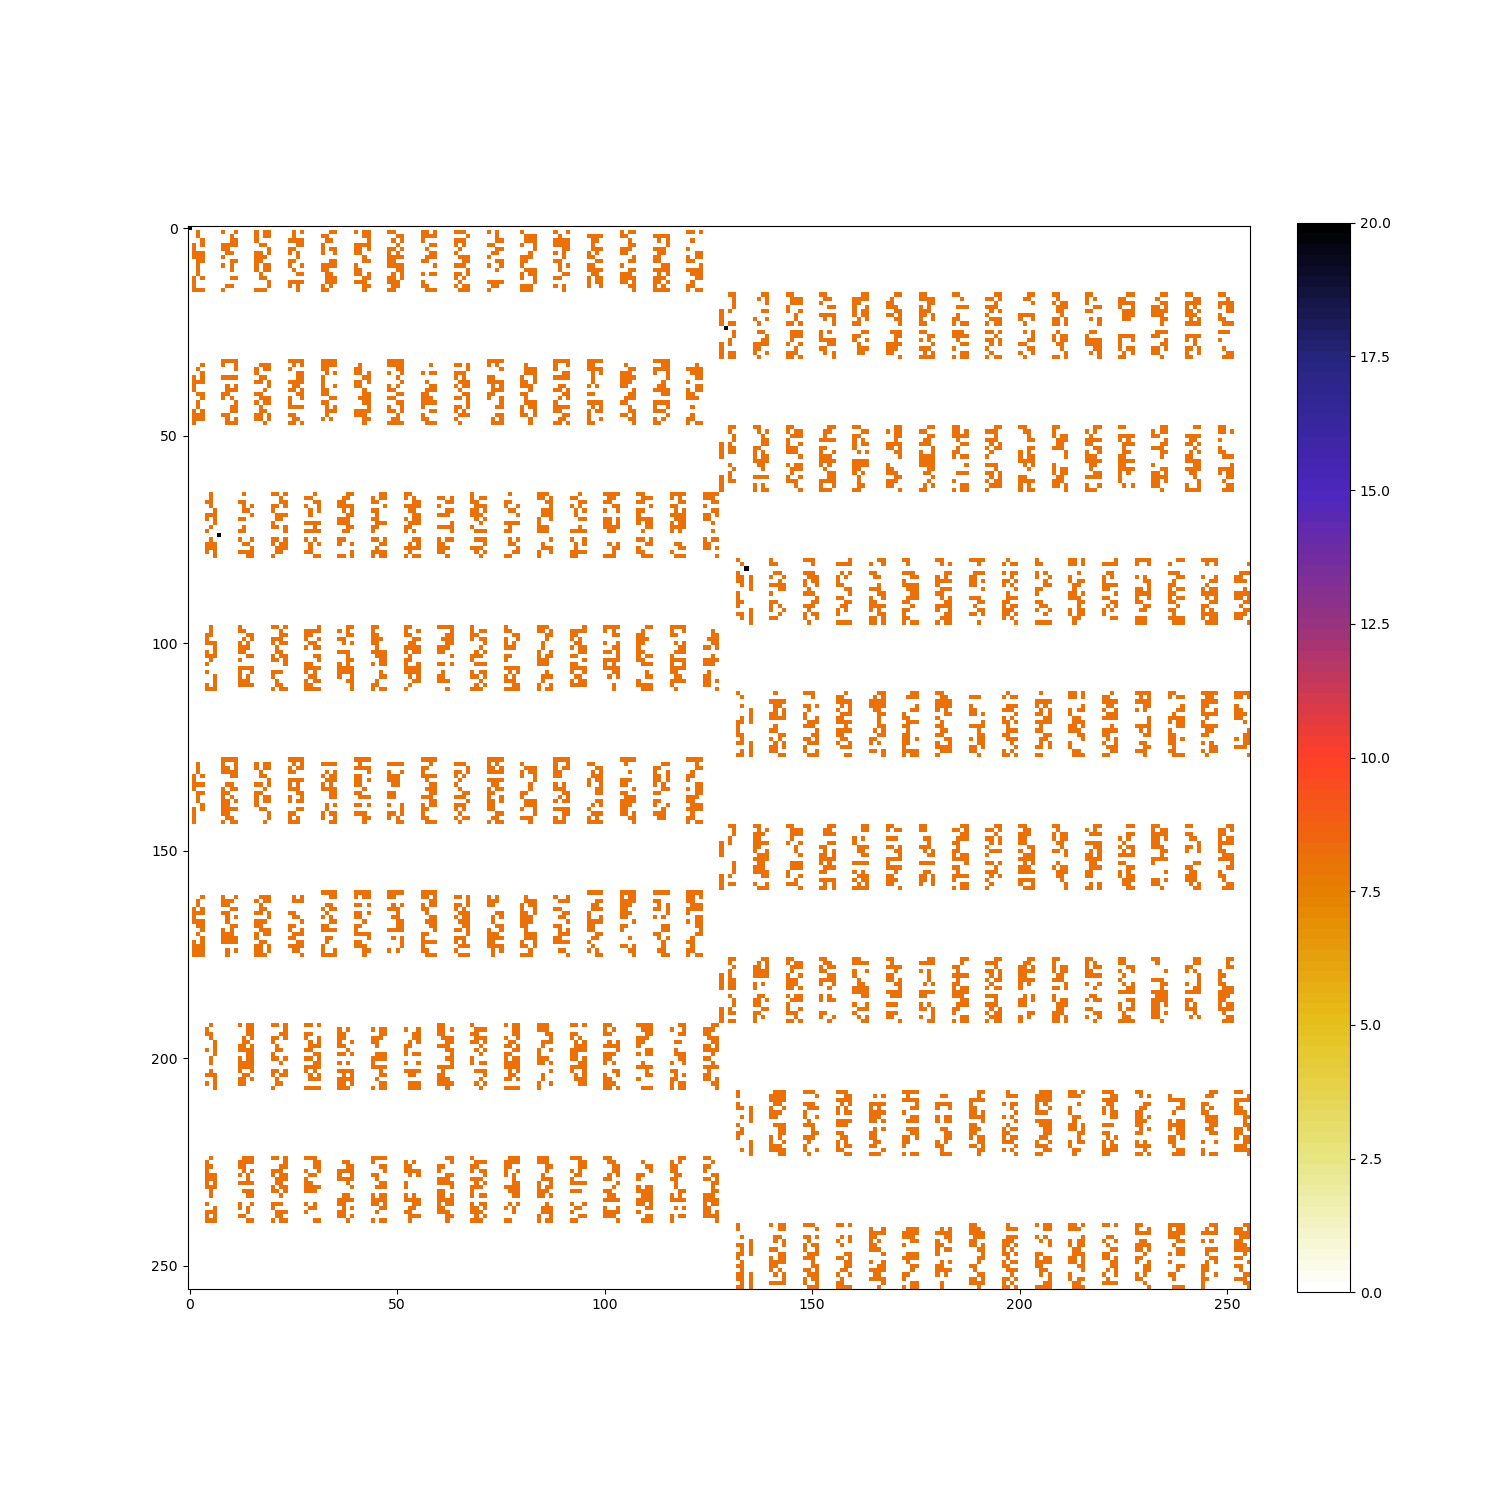
\includegraphics[trim=30pt 30pt 30pt 100pt, clip, width=0.9\textwidth]{img/crypto/jafar/sbox-ddt.png}
        \end{center}
    \end{columns}

\end{frame}



\begin{frame}{Introduire une différentielle}
        \begin{center}                  
            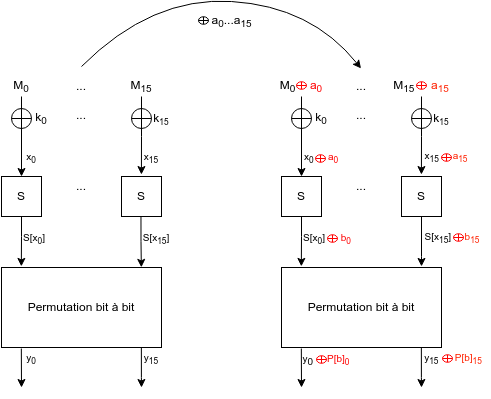
\includegraphics[width=0.53\textwidth]{img/crypto/jafar/auto/1round.png}
        \end{center}
        \pause
    \begin{itemize}
        \item $D_{in}=[0, 82, 0, 24, 0, 0, 0, 82, 0, 0, 0, 0, 0, 0, 0, 0]$
        \item $D_{out}=[0, 0, 0, 0, 0, 74, 0, 0, 0, 0, 24, 0, 0, 74, 0, 0]$
    \end{itemize}

\end{frame}


\begin{frame}{Sur 20 rounds}
        \begin{center}                  
            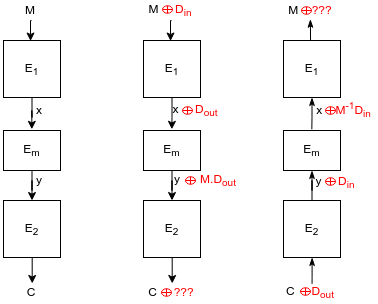
\includegraphics[width=0.6\textwidth]{img/crypto/jafar/auto/first-try.png}
        \end{center}
\end{frame}

\begin{frame}{Introduction au boomerang \only<6>{\flag}}
    \only<1>{
        \begin{center}                  
            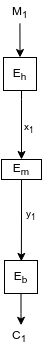
\includegraphics[scale=0.5]{img/crypto/jafar/auto/boomerang-1.png}
        \end{center}
    }
    \only<2>{
        \begin{center}                  
            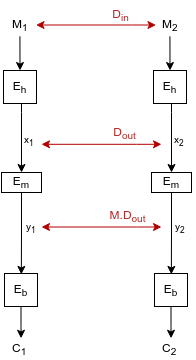
\includegraphics[scale=0.5]{img/crypto/jafar/auto/boomerang-2.png}
        \end{center}
    }
    \only<3>{
        \begin{center}                  
            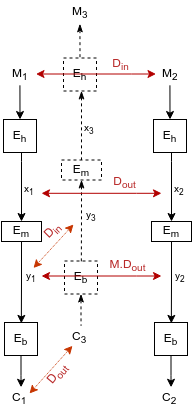
\includegraphics[scale=0.5]{img/crypto/jafar/auto/boomerang-3.png}
        \end{center}
    }
    \only<4>{
        \begin{center}                  
            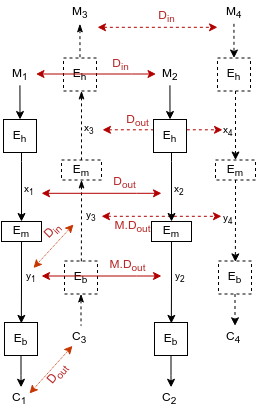
\includegraphics[scale=0.5]{img/crypto/jafar/auto/boomerang-4.png}
        \end{center}
    }
    \only<5->{
        \begin{center}                  
            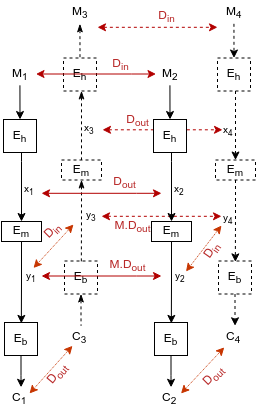
\includegraphics[scale=0.5]{img/crypto/jafar/auto/boomerang-5.png}
        \end{center}
    }

\end{frame}